\documentclass{article}
\usepackage{stmaryrd}
\usepackage{graphicx}
\usepackage{float}
\usepackage{caption}
\usepackage{subcaption}
\usepackage[colorlinks=true,allcolors=blue]{hyperref} % Ajout du package hyperref pour les liens
\title{Report, Kinetic project}
\author{Dorian Geraldes Pereira, Axel Demuth}
\date{March 2024}

\begin{document}
\maketitle
\tableofcontents
\newpage

\section{Introduction}

Our project is part of a larger initiative aimed at processing 
IFC files representing buildings to create 3D models for energy 
simulations with high-performance calculations.

\subsection{Project Objective}

Within this project scope, the primary goal is to implement an efficient and accurate 
conversion process for Industry Foundation Classes (IFC) 
files representing buildings or cities into meshes compatible with the 
Kinetic algorithm. Subsequently, the Kinetic algorithm will be applied to these 
meshes to produce watertight models, facilitating the execution of finite element calculations.

The specific steps to be undertaken are as follows:

\begin{enumerate}   
    \item \textbf{Reading Process or Mesh Conversion :} From the IFC files we will have a 
    conversion in the stl or msh format,we will need to change the reading process to be able 
    to read mesh from those format if possible,if we cant then we will convert the STL 
    or MSH meshes into one of the formats accepted by the Kinetic algorithm, 
    such as .ply, .xyz, .las, .off.
    
    \item \textbf{Application of the Kinetic Algorithm:} Applicate  
    the Kinetic algorithm on the the converted 
    meshes to produce meshes optimized for finite element calculations.
    
    \item \textbf{Recovery of Material Labels:} Ensure the preservation 
    of information regarding materials present in the initial IFC-format mesh 
    and correctly associate them with elements of the converted mesh.
    
    \item \textbf{Utilization on City Modeling:} Extend the application of 
    the Kinetic algorithm to entire city models.
\end{enumerate}

\subsection{Project Challenges}

Currently, the project faces several technical challenges:

\begin{enumerate}
    \item \textbf{Generating point cloud from stl file:} To use the kientic algorithm we need a point cloud format with normal on each point, 
    currently the result we get from the transformation arent satisfactory we need to find a solution to improve this conversion
    
    \item \textbf{Parameter Optimization:} Identify and adjust appropriate 
    parameters to avoid segmentation faults and achieve satisfactory results 
    when applying the Kinetic algorithm.
\end{enumerate}

By overcoming these challenges, the project aims to provide a 
comprehensive and efficient solution for analyzing urban structures 
using the Kinetic algorithm to facilitate finite element calculations.\newline

\section{Tools}
\subsection{CGAL}
CGAL is a comprehensive package for geometry algorithms, providing various data structures and algorithms for working on polygons, surfaces, mesh generation, and more.
It offers a wide range of functionalities for geometric processing and analysis in various fields such as computer graphics, computational geometry, and geometric modeling.
\subsection{IFC Format}

The initiative was created by buildingSMART (BIM), with the goal of supporting portability between software in the construction sector.
 IFC is a file format designed to replace a fragmented information system with a standardized one.
  This enables every actor in the sector to utilize IFC-compatible software to open files and model their contents without wasting time and computational resources on convertion between different formats.

The IFC format is a volume-based 3D representation , The file is very similar to object-oriented code, with numerous classes associated with various needs such as construction sites, tools, and materials.
However, a challenge we face is the difficulty in interpreting IFC objects for use in Kinetic programs. While there are several software solutions available to convert IFC to the desired format, 
we often lose significant amounts of information in the process.

As a result, we need to focus on refining the objects received from the converting process to ensure that Kinetic algorithm can effectively read the files.

\subsection{Kinetic}

Kinetic algorithm(KSR) is a package from CGAL that allows working on meshes with 
some holes in them. When applied to the mesh, the Kinetic algorithm will 'extend' some surfaces to fill the mesh and make it watertight. 
Here's what the algorithm is capable of:


\begin{figure}[H]
    
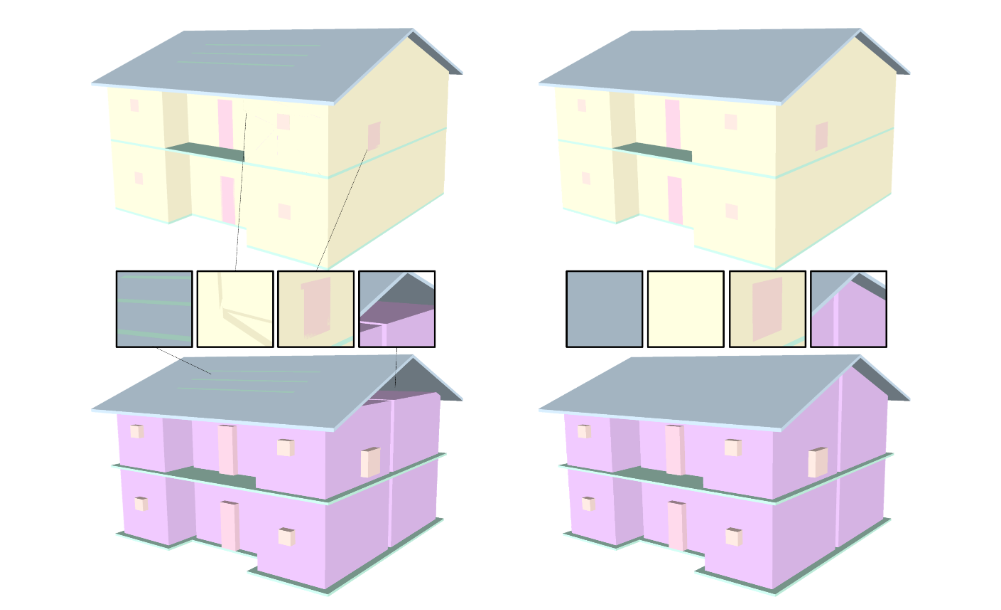
\includegraphics[scale =   0.3 ]{../../images/example_algorithm.png}

\end{figure}


\section{Implementation}

We are using the most complete example of the cgal kinetic algorithm as base for our main. In this main we can change every parameters of the algorithm.
\newline
To use the algorithm we currently need to give him a file from supported format such as .ply , .off, .xyz, .las .
Our main is now able to read STL and MSH format but for now by transorming the point of the format in an xyz file,
for now the result of this transformation is still bad because of the density of point given by the transformation compared to the density needed by the algorithm.
If the parameters dont respect the critera we described in the previous section the algorithm can end up in segmentation fault.
The result of the algorithm will be in an .off format in "resultat" folder.
\newline
We can present an example of the command to execute the program:
\newline
" ./build/default/bin/kinetic -data data/flame.ply -dist 0.3 -minp 50 -regangle 5 "
\newline


\subsection{File Format}
In this project we use different files Format as: 

\begin{itemize}
  \item XYZ : An XYZ file contains point cloud data with each point's coordinates in 3D space.
  \item PLY : A PLY file stores 3D model data including vertices, faces, and optional attributes like color and normals.
  \item STL : An STL file represents the surface geometry of a 3D object using triangular facets.
  
\end{itemize}

\subsection{STL Reading and Use}

In the CGAL library, we have methods to read various file formats such as PLY, OFF, and XYZ, including STL files. When we use the `read stl` function, we obtain the following output:

\begin{itemize}
  \item A list of all points used in the mesh.
  \item A list of vertices with all points used in every polygon.
\end{itemize}

Thus, we have access to a point cloud and a list of polygons. The KSR algorithm only needs a point cloud to work. We proceed by calculating the normals associated with all points, 
writing all the points and normals into an .xyz file, and then reading the .xyz file with our main program to apply the KSR algorithm.
However, one issue with STL files is the low number of points they provide, which leads to suboptimal performance of the algorithm and potential errors. Therefore, we need to find a way to densify our point cloud.
To execute KSR on our files, we tried different options:

\begin{itemize}
  \item Using free and open source software such as CloudCompare.
  \item Using CGAL methods to densify our point cloud, such as the CGAL Poisson surface reconstruction.
  \item Using Meshlab sampling functions as Monte Carlo sample or Poisson dist Sample
\end{itemize}


\subsection{Kinetic algorithm}
We can obtain a comprehensive understanding of how it works in general from the report by INRIA \cite{yu:hal-03621896}.

\begin{itemize}
\item It uses geometric primitives to create planes due to their relevance in human-made environments.
\item There are multiple methods for plan fitting in a 3D model, such as Neural Network architectures or Energy-based Models. The algorithm employs the latter.
\item To evaluate the quality of a primitive configuration x with an energy U of the format
  \newline 
  $        U(x) = w_f U_f(x) + w_s U_s(x) + w_c U_c(x)       $
  \newline
  where all U functions pertain to fidelity, simplicity, and completeness, and all w are positive and weight.
  \item It then utilizes geometric operations such as merging, splitting, transfer, insertion, and exclusion on different planes and closed primitives.
\end{itemize}
  Here, we present pseudocode detailing how the exploration of the set of primitives works:
\begin{center}
  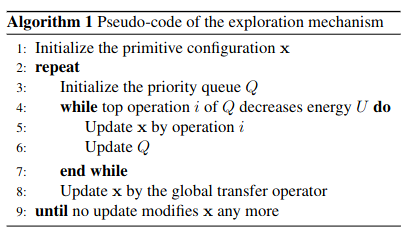
\includegraphics[scale =  0.5]{../../images/Pseudo_code_exploration.png}
\end{center}
The priority queue represents the set of primitives to which we apply geometric applications.

To use the algorithm, we employ one from CGAL. Given a set of parameters and a file containing a point cloud along with the associated normals to the points,
the algorithm is applied. We were fortunate to have a meeting with Florent Lafarge, one of the creators of the algorithm,
who explained to us which parameters are crucial for analysis and how each one can significantly influence the results.
Two parameters stand out as particularly important: 
\begin{itemize}
  \item 'dist' indicates the distance between two points required to consider them for plane construction.
  \item 'pmin' represents the number of points used to construct a plane.
\end{itemize}


\subsection{Data}
We obtained our different meshes from different sources with the name of the files: 
\begin{itemize}
  \item from the KSR example package from INRIA : flame.ply
  \item from the package \texttt{data\_point\_3} from CGAL : building.ply 
  \item from Vincent Chabannes : 3zones.stl , ACJasmin.stl
\end{itemize}

\subsection{Test of the parameter}
In order to understand how these parameters affect the outcome, we will examine the same point cloud while varying the value of 'pmin' first and then varying 'dist.'
The algorithm produces .off files as output, which can be visualized using software such as MeshLab.

\newpage
The original point cloud represents this building :
\vspace{\baselineskip}

\begin{center}
    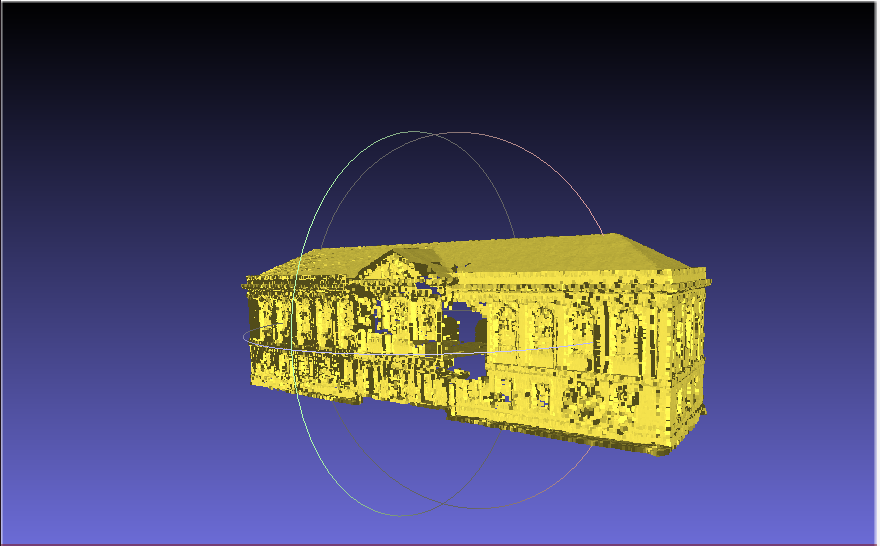
\includegraphics[scale=0.20]{../../images/screen_kinetic/building.png} 
\end{center}



\begin{figure}[H]
  \centering
  \begin{subfigure}[b]{0.45\textwidth}
    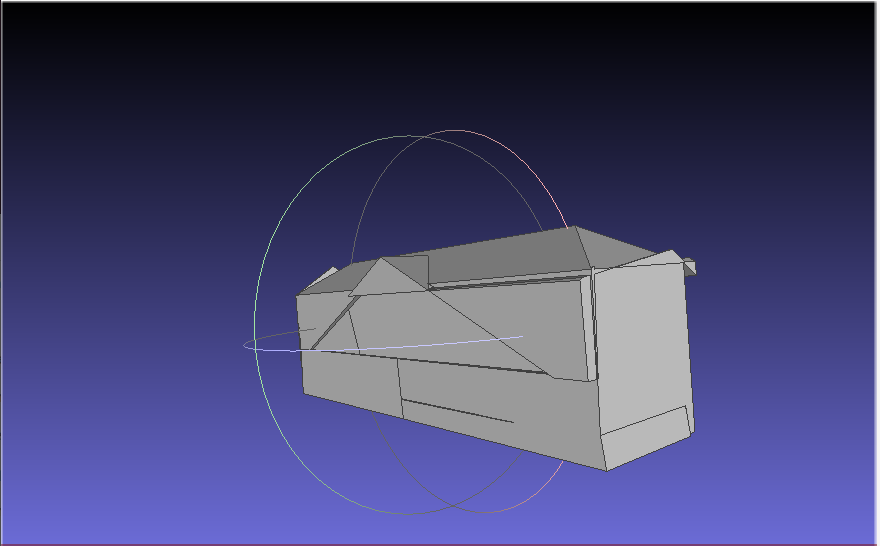
\includegraphics[width=\textwidth]{../../images/screen_kinetic/dist1_pmin220.png}
    \caption{dist1\_pmin220}
    \label{fig:dist1_pmin220}
  \end{subfigure}
  \hfill
  \begin{subfigure}[b]{0.45\textwidth}
    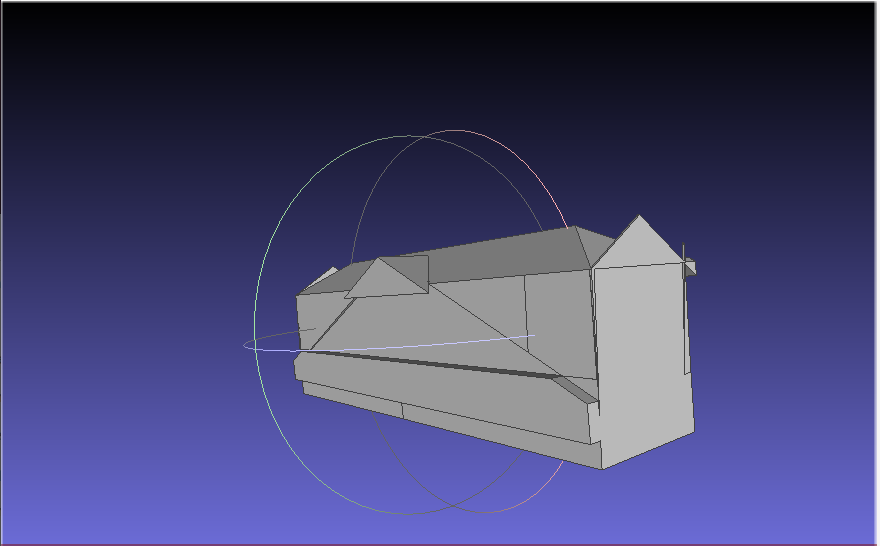
\includegraphics[width=\textwidth]{../../images/screen_kinetic/dist1_pmin250.png}
    \caption{dist1\_pmin250}
    \label{fig:dist1_pmin250}
  \end{subfigure}
  \vfill
  \begin{subfigure}[b]{0.45\textwidth}
    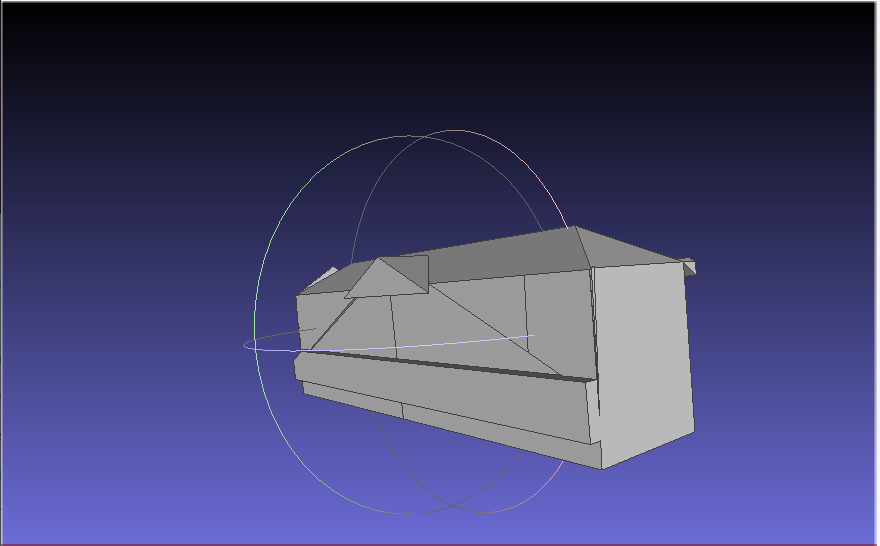
\includegraphics[width=\textwidth]{../../images/screen_kinetic/dist1_pmin280.png}
    \caption{dist1\_pmin280}
    \label{fig:dist1_pmin280}
  \end{subfigure}
  \hfill
  \begin{subfigure}[b]{0.45\textwidth}
    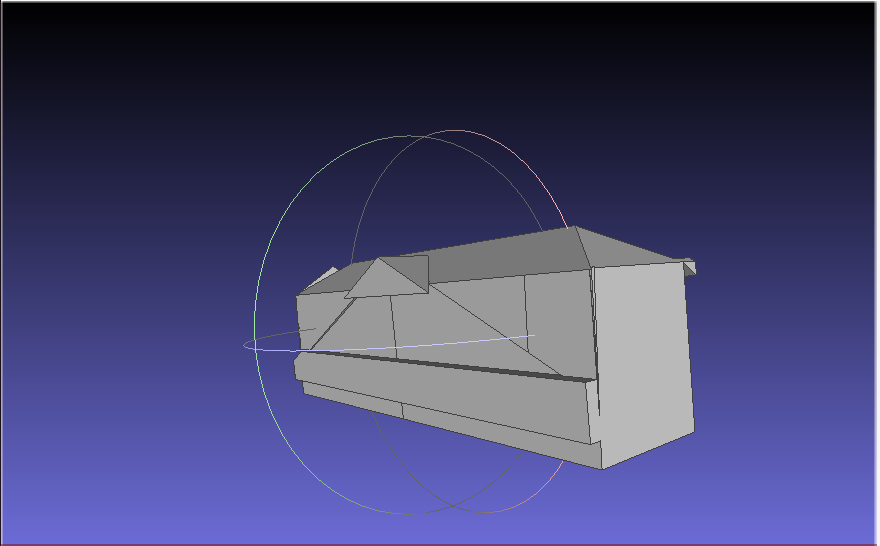
\includegraphics[width=\textwidth]{../../images/screen_kinetic/dist1_pmin300.png}
    \caption{dist1\_pmin300}
    \label{fig:dist1_pmin300}
  \end{subfigure}
  \caption{Variation of p\_min on the same mesh}
  \label{fig:ensemble_images}
\end{figure}
  
  First, it's important to understand that setting 'pmin' too low can lead to errors. Subsequently,if 'pmin' is too small, we may not capture enough structural detail,
  whereas setting 'pmin' too high may cause planes to overlap, resulting in loss of information



  \begin{figure}[H]
    \centering
    \begin{subfigure}[b]{0.45\textwidth}
      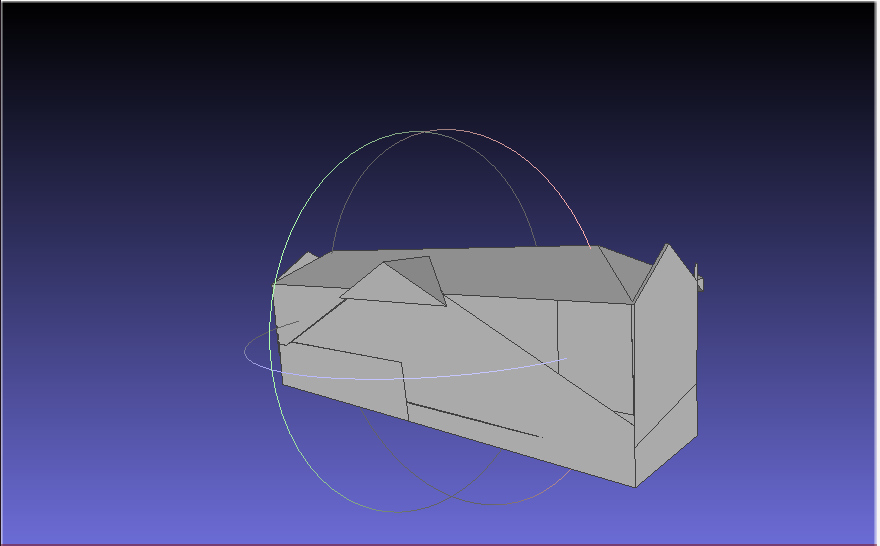
\includegraphics[width=\textwidth]{../../images/screen_kinetic/dist1_5_pmin_250.png}
      \caption{dist15\_pmin250}
      \label{fig:dist15_pmin220}
    \end{subfigure}
    \hfill
    \begin{subfigure}[b]{0.45\textwidth}
      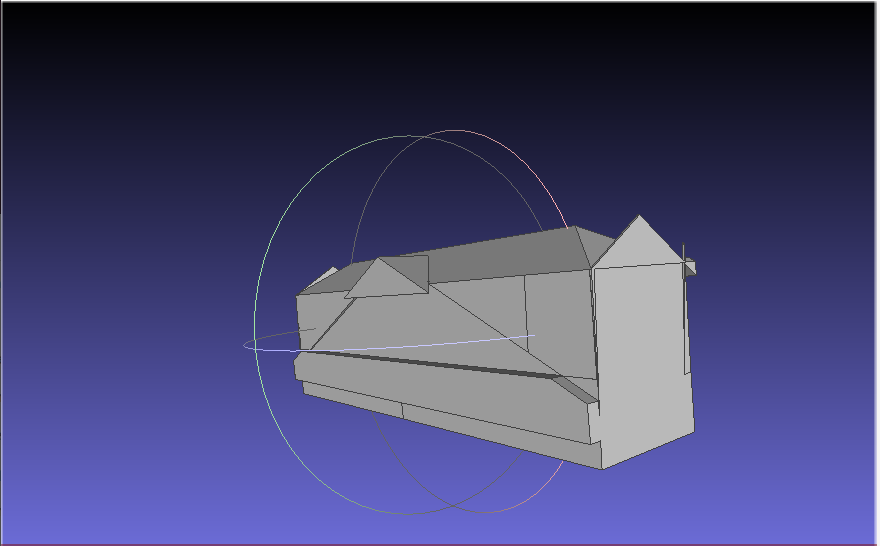
\includegraphics[width=\textwidth]{../../images/screen_kinetic/dist1_pmin250.png}
      \caption{dist1\_pmin250}
      \label{fig:dist1_pmin250}
    \end{subfigure}
    \vfill
    \begin{subfigure}[b]{0.45\textwidth}
      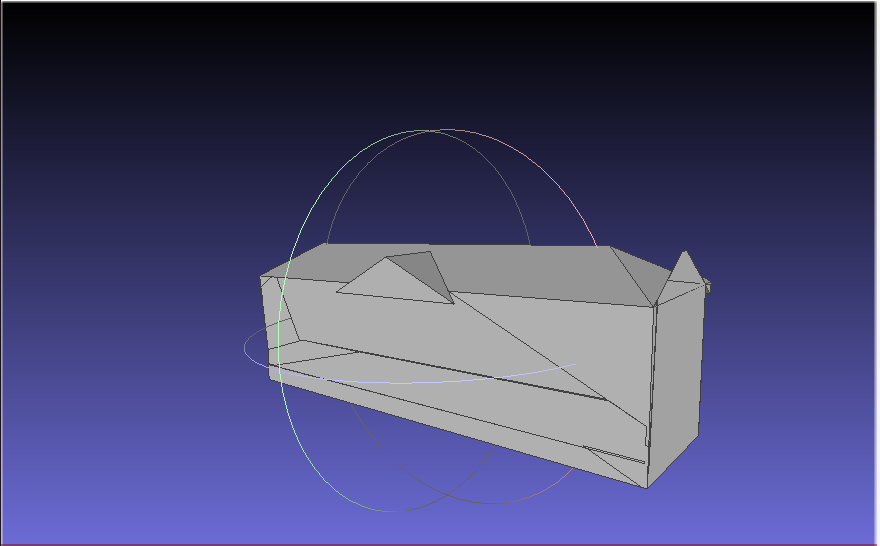
\includegraphics[width=\textwidth]{../../images/screen_kinetic/dist_0_3_pmin_250.png}
      \caption{dist0.3\_pmin250}
      \label{fig:dist0.3_pmin250}
    \end{subfigure}
    \hfill
    \begin{subfigure}[b]{0.45\textwidth}
      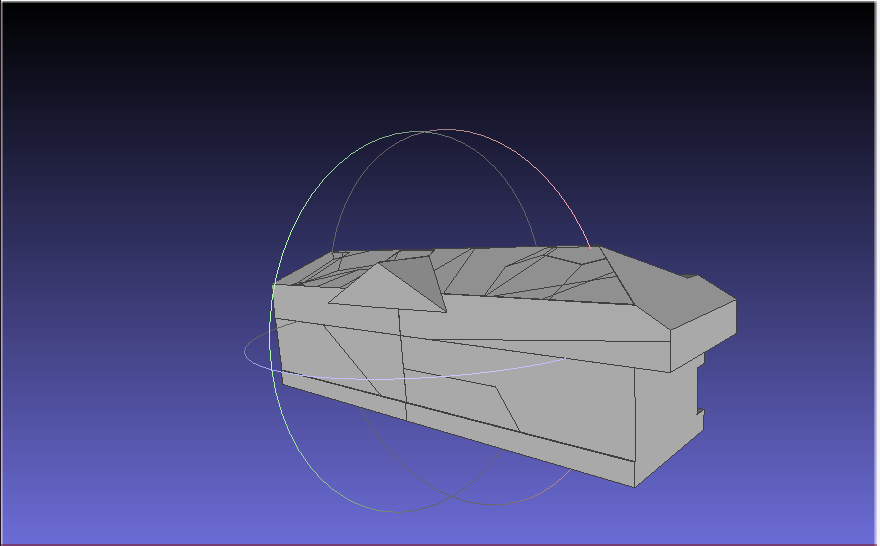
\includegraphics[width=\textwidth]{../../images/screen_kinetic/dist_001_pmin_250.png}
      \caption{dist0.01\_pmin250}
      \label{fig:dist0.01_pmin300}
    \end{subfigure}
    \vfill
    \begin{subfigure}[b]{0.45\textwidth}
      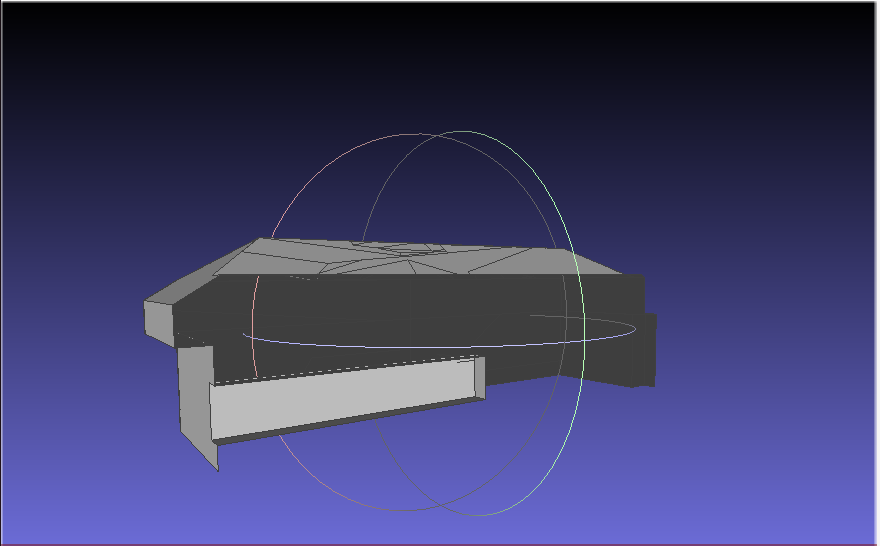
\includegraphics[width=\textwidth]{../../images/screen_kinetic/back_dist001_pmin250.png}
      \caption{back\_dist0.01\_pmin250}
      \label{fig:back_dist0.01_pmin250}
    \end{subfigure}
    \caption{Variation of dist on the same mesh}
    \label{fig:variation_pmin}
\end{figure}

  When considering the 'dist' parameter, if it is set too high, we risk losing significant structural details. 
  In the opposite, if the distance is too small, surfaces may be divided into too many planes, potentially resulting in an incomplete coverage of the entire mesh, 
  as observed at the rear of the building with a 'dist' of 0.001.

  One of the challenges in studying this algorithm is determining the appropriate 'qmin' and 'dist' to achieve the desired number of space partitions.
  Setting it too high may enhance precision but extend execution time, and in some cases, incorrect values can lead to program crashes.

This algorithm could be a crucial tool in our project, particularly when dealing with massive meshes for large buildings,
hospitals, etc. When creating large meshes, issues can arise, and errors within the mesh can be detrimental during simulations,potentially leading to false results. 
This algorithm allows us to rectify such mesh problems.

One limitation of the algorithm is its input requirement, as it currently only works with scatter plots. Consequently, we are unable to utilize the IFC format, 
resulting in the loss of valuable information regarding the types of structures present. To address this limitation, 
we plan to implement a process involving the conversion of IFC to scatter plot with associated data, followed by conversion to formats such as .plt, .ply, .xyz,
which are supported by Kinetic CGAL, ultimately resulting in a mesh with associated data.


\subsection{CloudCompare}
We used CloudCompare to create a densified point cloud with an stl file as basis.
This software can also calculate normals of each point, we used it sometimes to 
see the differences with cgal and meshlab because the normals of the point are very important to get the best result possible 

\subsection{CGAL Methods}
CGAL offers multiple ways to generate point clouds in theory. For example:

\begin{itemize}
  \item $CGAL::Spatial\_sort\_traits\_adapter\_3$ and $CGAL::natural\_neighbor\_coordinates\_3()$, interpolation methods like least squares or spatial interpolation.
  \item $CGAL::Delaunay\_triangulation\_3$ for triangulation of a mesh.
  \item $CGAL::point\_generators\_3::regular\_grid\_points()$ for generation on a grid.
\end{itemize}

If we succeed in generating a sufficiently large point cloud with one of these functions, we could try to write it in OFF, XYZ, or PLY files to read them and attempt to assemble the mesh to achieve the desired result.
 However, even if we manage to build our programs using one of these functions, we do not always get the results we want.
  For example, to use the neighbor coordinates, we first need to perform Delaunay triangulation. However, one problem with our STL file is that it's a non-oriented mesh, 
  so CGAL cannot calculate the Delaunay triangulation. Another problem is meshes with stairs, which implicate many points close to each other, causing errors in the generation process.



\section{Analysis of results}
\subsection{first results}
Analysis of the meshes reveals significant differences between those produced by the CGAL algorithm and those generated by the INRIA algorithm. The mesh obtained with CGAL demonstrates satisfactory watertightness but is characterized by noticeable roughness. Conversely, the mesh generated by the INRIA algorithm is remarkably smoother, offering a more uniform surface.

For better visual understanding, three images are provided below:

\begin{itemize}
    \item Initial point cloud
    \item Result of the mesh with the CGAL algorithm
    \item Result of the mesh with the INRIA algorithm
\end{itemize}

\vspace{0.5cm}
\begin{figure}[H]
  \centering
  \begin{minipage}[t]{0.29\textwidth}
  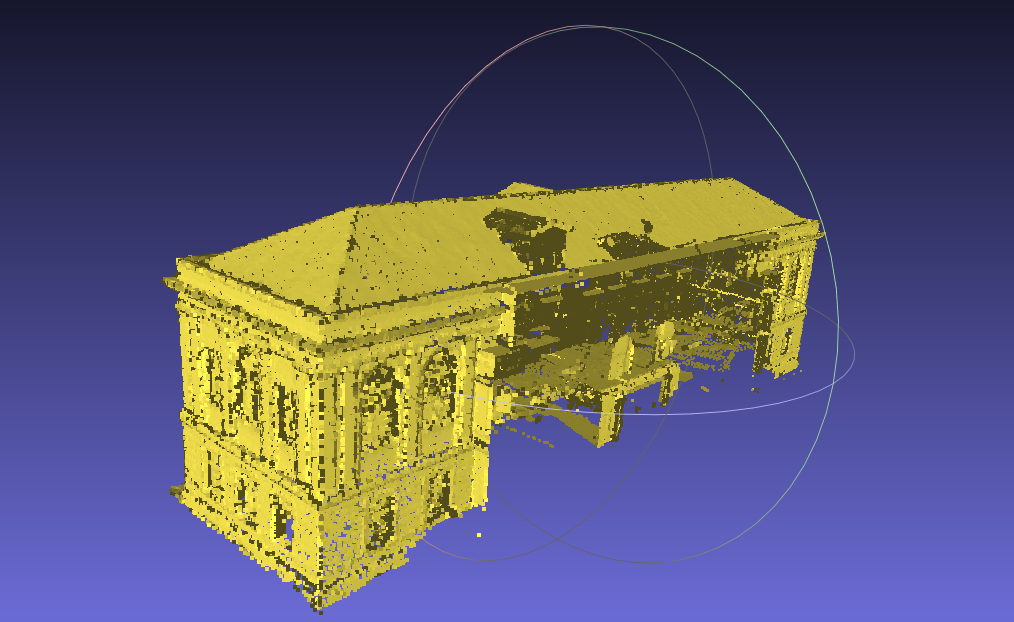
\includegraphics[width=\textwidth]{../../images/screen_kinetic/building_point.png}
  \caption*{point cloud,\newline
  file: building.ply}
\end{minipage}
  \begin{minipage}[t]{0.29\textwidth}
  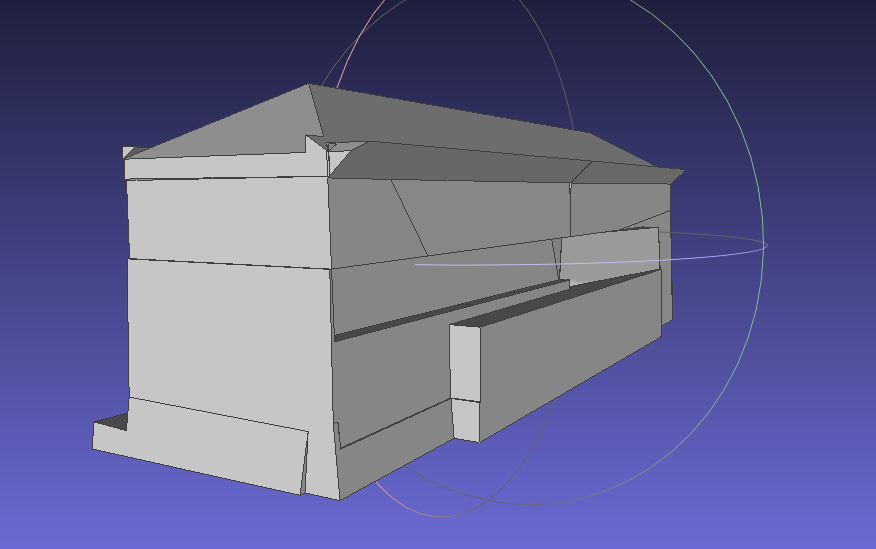
\includegraphics[width=\textwidth]{../../images/screen_kinetic/building_cgal.png}
  \caption*{cgal result,\newline
  data: building.ply, 
  \newline parameters: -dist 0.4 \newline-minp 100 -regangle0 5}
\end{minipage}
\hspace{0.05\textwidth}
  \begin{minipage}[t]{0.29\textwidth}
  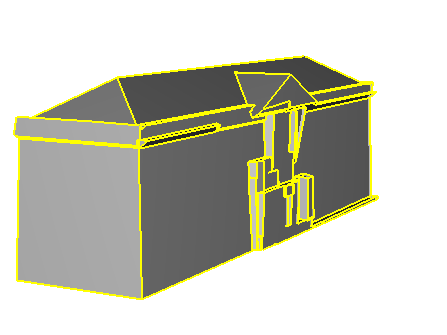
\includegraphics[width=\textwidth]{../../images/screen_kinetic/building_inria.png}
  \caption*{inria result,\newline
  data: building.ply
  }
  \end{minipage}
  \caption{Visualization of results with building.ply}
  \end{figure}
  \begin{figure}[H]
    \begin{minipage}[t]{0.29\textwidth}
        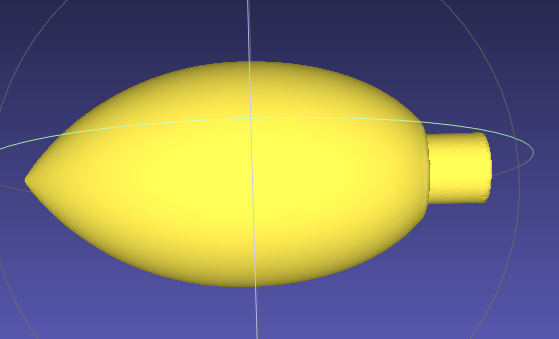
\includegraphics[width=\textwidth]{../../images/screen_kinetic/flame_point.png}
        \caption*{point cloud,\newline
        file: flame.ply}
    \end{minipage}
    \begin{minipage}[t]{0.33\textwidth}
      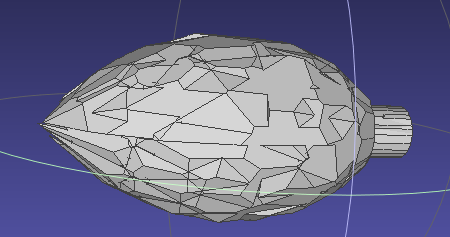
\includegraphics[width=\textwidth]{../../images/screen_kinetic/flame_cgal.png}
      \caption*{cgal result,\newline
      data: flame.ply}
    \end{minipage}
    \begin{minipage}[t]{0.27\textwidth}
        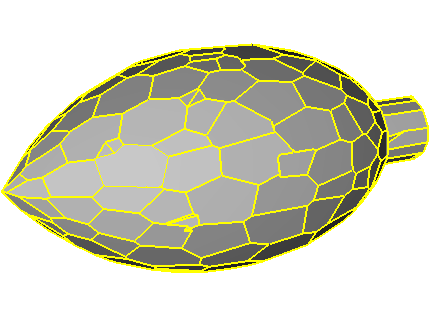
\includegraphics[width=\textwidth]{../../images/screen_kinetic/flame_inria.png}
        \caption*{inria result,\newline
        data: flame.ply}
      \end{minipage}
      \caption{Visualization of results with flame.ply}
\end{figure}

\subsection{Final Result}

For the final analysis we worked on 2 of the example provided by Vincent Chabannes:
\vspace{0.5cm}
\begin{figure}[H]
  \centering
  \begin{minipage}[t]{0.29\textwidth}
    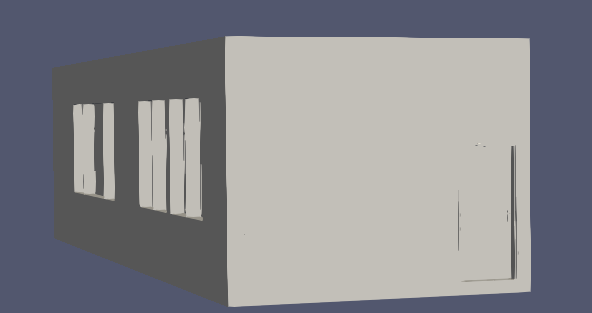
\includegraphics[width=\textwidth]{../../images/screen_kinetic/3zones.png}
    \caption*{3zones}
  \end{minipage}
  \hspace{0.05\textwidth}
  \begin{minipage}[t]{0.27\textwidth}
    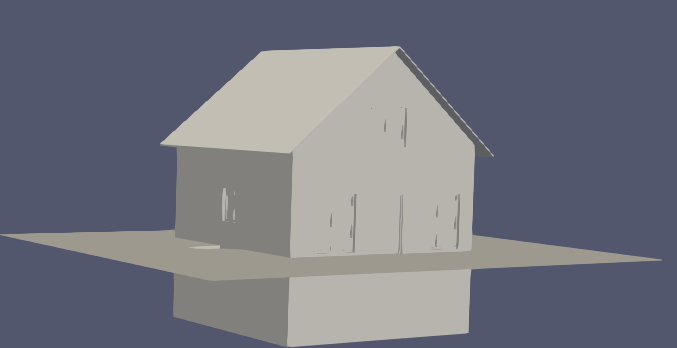
\includegraphics[width=\textwidth]{../../images/screen_kinetic/ACJasmin.png}
    \caption*{ACJasmin}
  \end{minipage}
  \hspace{0.05\textwidth}
  \begin{minipage}[t]{0.27\textwidth}
    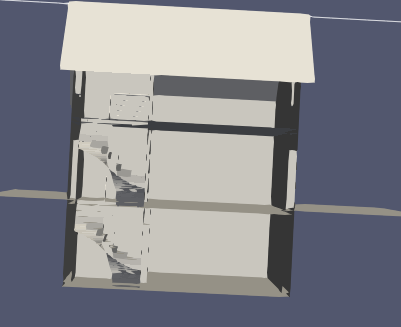
\includegraphics[width=\textwidth]{../../images/screen_kinetic/ACJasmin_inside.png}
    \caption*{ACJasmin\_inside}
  \end{minipage}
  \caption{Visualization of STL files that serves as basis for the following example}
\end{figure}  

For the first example, 3zones, 
we used CloudCompare to create the PLY point cloud file for the CGAL algorithm, 
and we calculated the necessary normals in Meshlab, which gave us the best results. 
However, the resulting watertight mesh lost all the details from the STL file,
such as the windows and doors, which have disappeared.
We can also see the importance of the normals calculation for the algorithm.

\vspace{0.5cm}
\begin{figure}[H]
  \centering
  \begin{minipage}[t]{0.32\textwidth}
    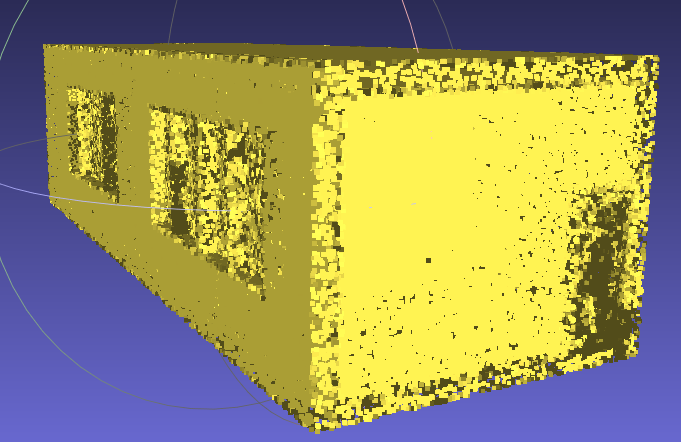
\includegraphics[width=\textwidth]{../../images/screen_kinetic/3zones_point_cloud.png}
    \caption*{point cloud}
  \end{minipage}

  \begin{minipage}[t]{0.35\textwidth}
    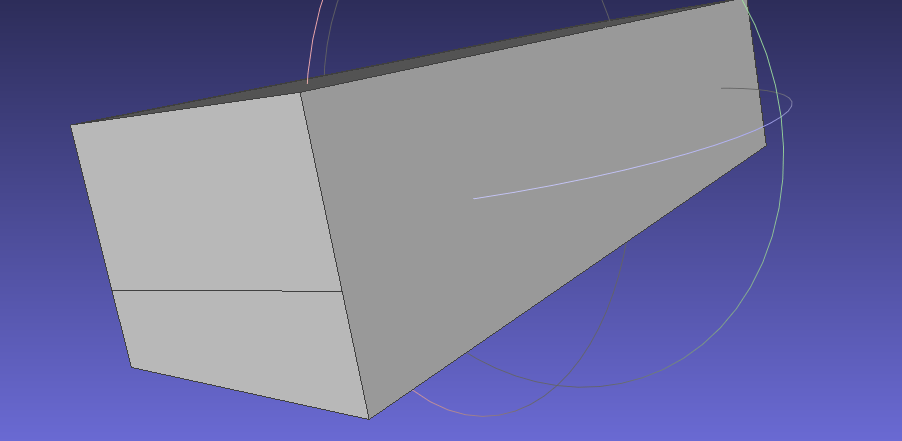
\includegraphics[width=\textwidth]{../../images/screen_kinetic/3zones_result_normal5_cgal.png}
    \caption*{result normal by MeshLab,\newline
    data: 3zones\_normal5.ply,\newline
    parameters: -dist 0.2 \newline-minp 500}
  \end{minipage}
  \hspace{0.05\textwidth}
  \begin{minipage}[t]{0.29\textwidth}
    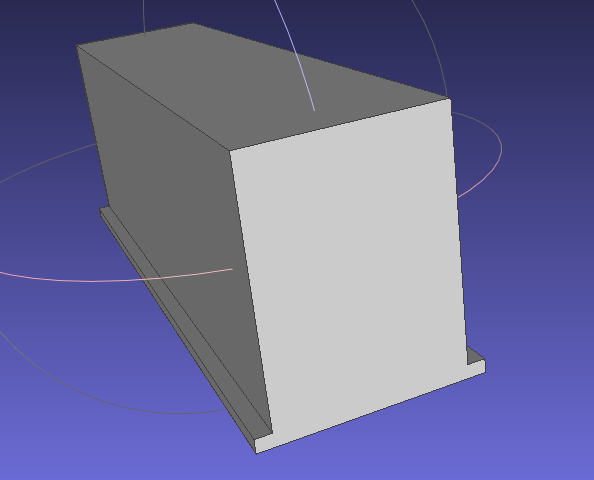
\includegraphics[width=\textwidth]{../../images/screen_kinetic/3zones_result_normal_cgal.png}
    \caption*{result normal by cgal,\newline data: 3zones\_normal\_apres.ply,\newline
    parameters: -dist 0.2 \newline-minp 500}
  \end{minipage}
  \caption{result with 3zones example}
\end{figure}  

For the second example, ACJasmin we used the same protocol as the first example but for 
this example we decided to remove the ground around the house because it created a lots of problems,
the result we got were a lot more disapointing than the first example.
The mesh we got is open and we lost nearly every detail like the first example 
just a bit of the stairs still remained
This is the result we got from the cgal version:
\vspace{\baselineskip}
\begin{figure}[H]
  \centering
  \begin{minipage}[t]{0.29\textwidth}
    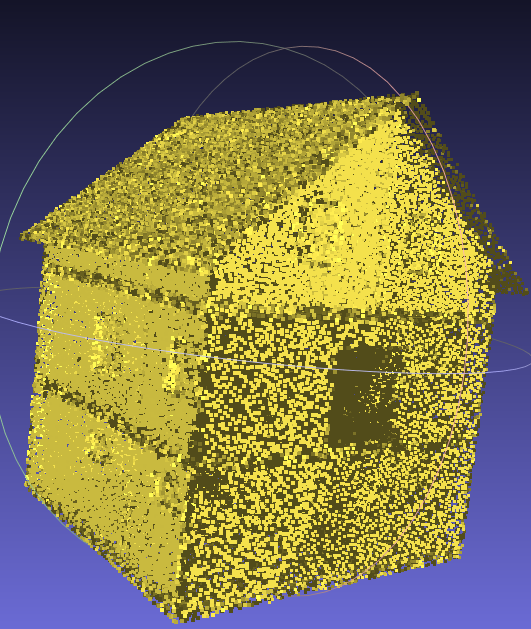
\includegraphics[width=\textwidth]{../../images/screen_kinetic/ACJasmin_point_cloud.png}
    \caption*{point cloud}
  \end{minipage}
  \hspace{0.05\textwidth}
  \begin{minipage}[t]{0.29\textwidth}
    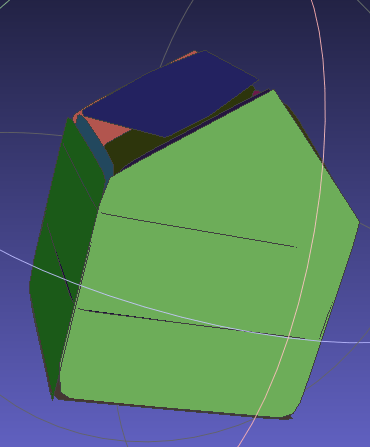
\includegraphics[width=\textwidth]{../../images/screen_kinetic/ACJasmin_primitive_cgal.png}
    \caption*{primitives}
  \end{minipage}
  \hspace{0.05\textwidth}
  \begin{minipage}[t]{0.27\textwidth}
    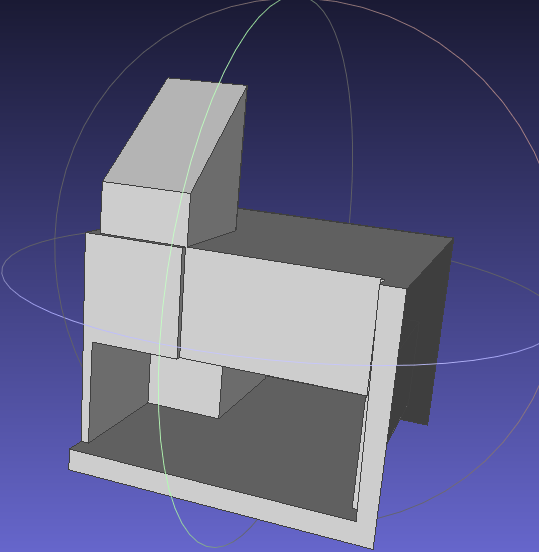
\includegraphics[width=\textwidth]{../../images/screen_kinetic/ACJasmin_result_CGAL.png}
    \caption*{result,
    \newline parameters: -dist 0.3 \newline-minp 300}
  \end{minipage}
  \caption{result of ACJasmin with cgal, data: ACJasmin\_Mesh.ply}
\end{figure}  

After the cgal version we tried the IRNIA version the result was still disapointing but better: 
\vspace{\baselineskip}
\begin{figure}[H]
  \centering
  \begin{minipage}[t]{0.29\textwidth}
    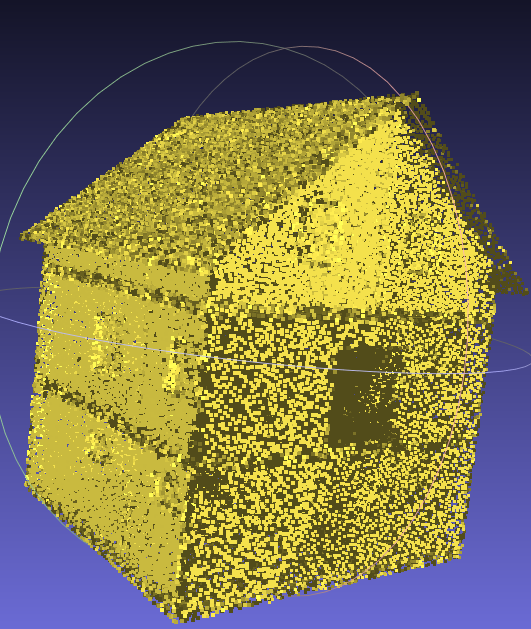
\includegraphics[width=\textwidth]{../../images/screen_kinetic/ACJasmin_point_cloud.png}
    \caption*{point cloud}
  \end{minipage}
  \begin{minipage}[t]{0.29\textwidth}
    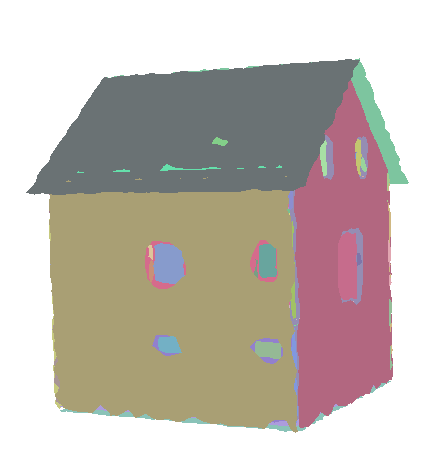
\includegraphics[width=\textwidth]{../../images/screen_kinetic/ACJasmin_primitive.png}
    \caption*{primitives}
  \end{minipage}
  \begin{minipage}[t]{0.27\textwidth}
    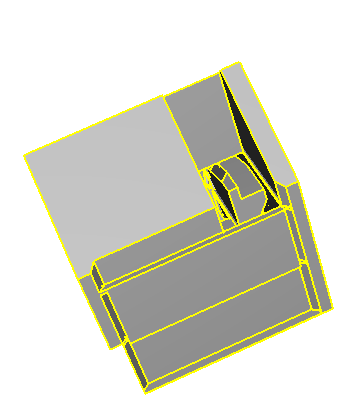
\includegraphics[width=\textwidth]{../../images/screen_kinetic/ACJasmin_result_INRIA.png}
    \caption*{result}
  \end{minipage}
  \caption{result of ACJasmin with cgal, data: ACJasmin\_Mesh.ply}
\end{figure}  
As we can see in those images the results we have from the 
algorithm isnt really satisfactory we need to find a solution 
to improve the quality of the outcome.


\section{Roadmap}
At this point those are the main Issues that we will need to work on:
\begin{itemize}
  \item Create better data to use the algorithm (mesh orientation and normal calculations)
  \item If possible, be able to retrieve the labels on the mesh generated by the Kinetic algorithm.
  \item Quality check of the obtained mesh from the kinetic algorithm (same volume as the first mesh)
  \item Apply physical theories to the base mesh and the output mesh to analyze the differences between them.
  \item Investigate the feasibility of applying the algorithm on a larger scale, such as a city or a large building, instead of a basic one.
\end{itemize}

For the V1 we modified and completed some issues:
\begin{itemize}
  \item The Issues Create watertight mesh with kinetic we completed what we wanted to do with this issue but now we want to go further so we modified it 
  to create watertight mesh from files coming to IFC format for the V2
  \item The issue Convert IFC to PLY format was also changed to change the reading process or convert MSH and STL to supported cgal format for the V2
  \item The issue setup programming environment for CGAL with github action and submodul,the creation of the main program,the study of the kinetic program were completed 
\end{itemize}



\section{Conclusion}
The kinetic algorithm serves the purpose of upgrading meshes and making them watertight, even if some details are lost in the process. However, 
there are still many limitations regarding its application, and significant preprocessing of the mesh may be required before executing the algorithm. 
Even after converting the STL mesh into a point cloud for the kinetic algorithm, the results are not satisfactory.

We can explore different ways to improve our results. Future work should focus on orienting the mesh from the STL file and generating a better point cloud. 
By ensuring the mesh is correctly oriented, we can effectively apply Delaunay triangulation or other CGAL methods without encountering errors to  generate a denser 
and more accurate point cloud will enhance the performance of the KSR algorithm and lead to better outcomes in our applications.

\nocite{*}
\section{Reference}
\bibliographystyle{plain}
\bibliography{../../bibliography/vfinal/report_bib}
\end{document}